\section{Problem definition} \label{problem}

In this chapter, we introduce the problem this thesis addresses and define the scope of our work. We also formalize the problem by formulating a research question, and present the approaches we will implement.

The problem, presented in section \ref{problem_intro}, arises from the poor quality of the subjects that are currently present in the repositories. 81 \% of all subjects are only assigned to one document, and only 5 \% of the subjects are assigned to more than three documents. This makes it hard to navigate the repositories by filtering the documents by subject, which is the purpose of having subjects. The sets of subjects are also different for each repository, which hinders the interoperability.

In section \ref{problem_scope} we define the scope of this thesis. We only consider the titles and abstracts of theses and publications written in English, which reduces the complexity of the task without hindering its research interest. We also restrict ourselves to evaluating methods that use an existing set of subjects. We use the subjects extracted from  the \acrfull{mag}, which is able to identify the relevant concepts in science because of its size. These subjects can then be used for any multidisciplinary repository, other than those included in our experiments.

Once the problem and scope have been introduced, we formalize the problem by formulating the research question this thesis attempts to answer, in section \ref{problem_rq}. This thesis focuses on the evaluation of supervised and unsupervised algorithms for performing \acrlong{si} in small and multidisciplinary repositories. 

\subsection{Introduction} \label{problem_intro}

As discussed in chapter \ref{repo_analysis}, the subjects that are currently present in the repositories are not well maintained. 81 \% of all subjects occur only once, i.e. they are only used by one publication. These cannot be used to relate documents. Furthermore, only 5 \% of the subjects are used by more than 3 publications. The poor quality of the subjects decreases the accessibility of the repositories. Each of them contains thousands of documents, and navigating them can be a cumbersome task. Subjects can be a useful tool for finding the desired documents, and also for looking for documents that are related to the ones we are currently reading.

Consider a repository where there is a maintained set of subjects. Each document in the repository is assigned a subset of these subjects, which can be navigated through the document's page in the repository. If a user is currently reading a publication about brain-computer interfacing, and would like to read more about that topic, the user could browse other documents that handle it by clicking on the corresponding subject. Furthermore, if the user has trouble understanding one of the building blocks of the documents, the user can click on the corresponding subject to search for other documents that maybe present that concept in more detail.
\subsection{Scope} \label{problem_scope}

Thus, our goal is to improve the quality of the \acrshort{si} in the repositories. In this section, we define the scope of this thesis. We do so before formulating the research question, as if not the problem is too broad and unclear.

Performing subject indexing in all the documents would require a lot of software engineering and special treatment of certain types of documents. This would hinder the scientific purpose of this thesis. We therefore start by considering which documents should be indexed in section \ref{problem_scope_docs}. Those documents will form our dataset. Then, in section \ref{problem_scope_asi}, we discuss which type of indexing methods will be implemented and evaluated in this thesis. We pick one of the two main paradigms of subject indexing and argue why it is better suited to our use case. Our approaches require a set of subjects, which they will assign to the documents of our dataset. We define this set in section \ref{problem_scope_subjects}. We explain several choices we have made, such as its size and composition.

\subsubsection{Documents} \label{problem_scope_docs}

The scope of this work are the publications and theses written in English. In the repositories there are also data files and other types of documents, but they are not suited for this work because of their lack of text and variety in format. Which document types are included in the dataset are shown in table \ref{tab:document_types}.

Only English documents (and English metadata, for that matter) are considered because it greatly reduces the complexity of the task and doing so does not seem to reduce the quality of the data. For example, out of the 28,720 documents present in the Free University's repository, 21,701 of them have the same number of English subjects as they have German subjects. A probable cause of this is that ones are the translations of the others. If this were the case, discarding the German subjects would not imply information loss. Also, adding other languages to the \acrshort{si} pipeline would not introduce any major changes in how we assign subjects to documents. There is therefore no research interest in doing so.

Instead of using the full texts of each document, we will only use the titles and the abstracts. This should reduce the computational cost of our approaches and also facilitate the encoding task, as only the most important aspects covered by the paper are taken into account. Using the full texts could potentially reduce the quality of the encodings, as they cover more topics. Especially theses, which sometimes comprise hundreds of pages and are broad in their content, would be expensive to process and hard to index.

We also harvest further metadata from the documents, such as subjects, publication venues, as well as the advisors and referees of theses. All these are used to create evaluation datasets, as explained in section \ref{eval_datasets}, and all except the subjects are also part of the unsupervised approach.

\begin{table}
\begin{center}
 \begin{tabular}{| c | c | c|} 
 \hline
 \thead{Kept?} & \thead{Group} & \thead{Types} \\ [0.5ex]
 \hline\hline
 \makecell{Yes} & \makecell{Thesis} & \makecell{Doctoral thesis, Bachelor thesis, Master \\ thesis, Study thesis, Habilitation} \\ 
 \hline
 \makecell{Yes} & \makecell{Publication} & \makecell{Preprint, Book part, Book, Article, \\ Conference proceedings, Conference \\ object, Periodical part, Working paper, \\ Research paper, Report} \\
 \hline
 \makecell{No} & \makecell{Data} & \makecell{Video, 3D Model, Textual data, Audio, \\ Sound, Moving image, Image, Dataset, \\ Generic research data, Research data} \\
 \hline
 \makecell{No} & \makecell{University} & \makecell{Course material, Lecture} \\
 \hline
 \makecell{No} & \makecell{Other} & \makecell{Draft, Software, Collection, Review, Other} \\
 \hline
\end{tabular}
\caption{All the document types present in the three repositories. The groups are only for clarity.}
\label{tab:document_types}
\end{center}
\end{table}
\subsubsection{Subject Indexing} \label{problem_scope_asi}

In chapter \ref{subject_indexing}, we discuss the different ways in which \acrshort{si} approaches can be classified. For now, we only require the distinction between \textit{assigned SI} and \textit{derived SI}, which differ on the subjects that are used to index the documents. In assigned \acrshort{si}, an existing set of subjects is used. The set can be constructed manually or retrieved from another application. On the other hand, derived \acrshort{si} extracts the subjects from the documents using only intrinsic information, such as term frequency.

Assigned \acrshort{si} is the preferred approach for information retrieval because it offers better precision and recall, given that users don't always know exactly the subjects they are looking for \cite{golub2019automatic}. Furthermore, using the same set of subjects in all three repositories allows them to be searched together. If each repository had its own set of subjects, their accessibility would be hindered. This is why standard sets of subjects, such as the \acrfull{ddc}, are so useful.

Given the heterogeneity and the technical nature of our dataset, derived \acrshort{si} approaches would not reach the desired quality. Our heterogeneous dataset limits the performance of term-weighting methods, such as TF-IDF, as phrases that are relevant because of their scientific meaning may not appear often enough to be noticed by these methods. Because of this, and given the availability of a suitable set of subjects, we will focus solely on methods that perform assigned \acrshort{si}. The existing subjects in the repositories will be used only for evaluation purposes.

We will use the subjects from \acrfull{mag}, a scientific knowledge graph presented in section \ref{subject_indexing_mag}. The set Microsoft has built covers all the disciplines present in the repositories and is therefore well suited for our task. It also includes a hierarchy, which we will use when training classification models. In the following section, we further discuss the \acrshort{mag} set of subjects. We argue why a subset of them suffices for our approach and which size and composition we require. We then present the final set of subject we use in this thesis.
\subsubsection{Set of subjects} \label{problem_scope_subjects}

Our dataset comprises considerably fewer documents than \acrshort{mag} (tens of thousands instead of hundreds of millions). Given that our goal is to relate documents to one another through their content, and we are focusing on small repositories, we don't require such granular subjects. If we used all the \acrshort{mag} subjects, most of them would be left unassigned, and many others would be assigned only once. We therefore pick a subset of these subjects.

\acrshort{mag} structures their set of subject as a hierarchy, where the first level comprises 19 subjects, which we call fields for clarity. Under each field, there exist five further hierarchy levels. We extract the subjects from OpenAlex, which is currently the best data source for subjects and publications of \acrshort{mag} (see section \ref{mag_access_data}).

In section \ref{problem_scope_subjects_retrieve}, we present our subject retrieval procedure. We discuss how many subjects we retrieve per field, and on what conditions we pick among the thousands of candidates. Then, we present the resulting set of subjects in section \ref{problem_scope_subjects_result}.

\paragraph{Subject retrieval} \mbox{} \label{problem_scope_subjects_retrieve}

We have extracted up to 200 descendants of each of the 19 fields. We consider how many publications a subject has been assigned to, assuming that popular subjects are more likely to appear in the repositories. We have tried different thresholds for how many assignments a subject needs to be considered, to strike a balance between picking subjects from the upper levels, which are more general, and picking subjects that are popular.

The problem is that the fields differ in popularity. For example, \textit{Medicine} has more than 200 subjects in the third level with more than 25k works, whereas \textit{Environmental science} only has 31 across all levels. We therefore start with a larger limit, iterate over all levels and all fields, and decrease the limit before iterating again. We first iterate through the descendants of each field and add subjects that are assigned to at least 25,000 publications. If the list of a field does not include 200 subjects after this iteration, we do so again, considering subjects assigned to at least 10,000. We repeat this procedure with 5,000, 1,000 and 100 assignments. When we iterate through the subjects of a field, we start by the second level and descend if necessary.

To avoid uninformative Wikipedia texts such as ``Emotionalism may refer to:'', we discard subjects whose description says ``Wikimedia disambiguation page'' or ``Wikimedia glossary list article''. The description from a subject comes from the corresponding Wikidata link, through which we later extract the Wikipedia link. For each subject that meets these requirements, we append it to all the fields it has in its list of ancestors, to keep the number of subjects as low as possible while providing good coverage of the fields.

\paragraph{Resulting set of subjects} \mbox{} \label{problem_scope_subjects_result}

\begin{figure}
    \centering
    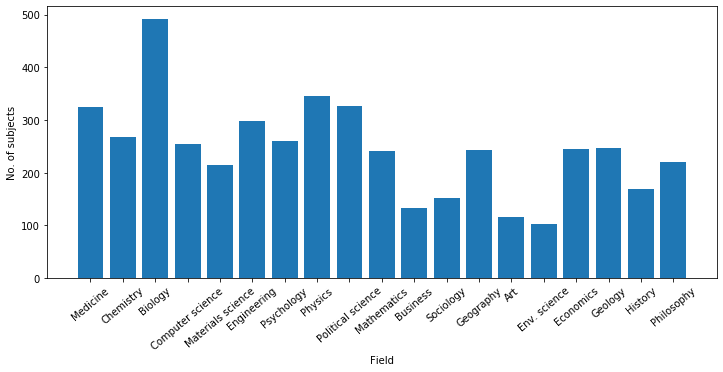
\includegraphics[width=\textwidth]{figures/unsupervised_approach/subjects_per_field.png}
    \caption{Number of subject that descend of each of the fields.}
    \label{fig:subjects_per_field}
\end{figure}

2,157 subjects were extracted with this procedure, which results on an average of 114 subjects per field. We could extract 200 subjects for all fields except for \textit{Environmental Science}, \textit{Business}, \textit{Sociology}, \textit{Art} and \textit{History}. On the other hand, \textit{Medicine}, \textit{Biology} and \textit{Physics} have more than 300 descendant subjects under the ones we have collected. This is because subjects can descend from multiple fields. For example, \textit{Neuroscience} can be classified under \textit{Biology}, \textit{Medicine} and \textit{Computer science}. The number of subjects per field can be seen in figure \ref{fig:subjects_per_field}.

All 25 subjects of the second level have been picked, followed by 1,999 of the third level, 108 of the fourth, and 6 of the fifth. On average, subjects are assigned to 197,180 publications. No subjects are assigned to less than 100 documents, as this was a requirement in the extraction procedure. Regarding the hierarchy of the subjects, all but 13 of them have ancestors in all levels above them. Two subjects of the third, \textit{Sensitivity} and \textit{Boundary}, are directly linked to fields. \textit{Sensitivity} is a descendant of both \textit{Engineering} and \textit{Mathematics}, whereas \textit{Boundary} descends from \textit{Mathematics}. The remaining eleven subjects that don't have ancestors in all previous levels belong to the fourth level. All of them descend from subjects of the second level, thus skipping the third level.
\subsection{Research question} \label{problem_rq}

The research question this thesis attempts to answer is the following:

\begin{quote}
    \textit{What family of approaches, supervised or unsupervised, is more suitable for performing subject indexing in small and multidisciplinary repositories?}
\end{quote}

The distinction between supervised and unsupervised is made in the field of machine learning, which is the paradigm we plan on implementing, as it is the most powerful method according to the literature (see chapter \ref{subject_indexing}).

Supervised approaches are those that learn through examples. They receive input-output pairs, and they are optimized to output what is expected for each of those inputs. The input-output pairs are usually called \textit{training data}, and the final performance of the model largely depends on its quality. Unsupervised approaches are fundamentally opposite: they learn to perform an action directly from the data, without any examples. They are based on the intuition that the data itself contains the necessary information for the model to perform its task
\cite{hinton1999unsupervised}.

Both approaches are interesting for our use case because of the size and content of our dataset. Supervised approaches have been proven more effective in most scenarios, and also in \acrshort{si} tasks. However, they require accurate training data, which is not available in our use case. The assignments of \acrshort{mag} are reported to be 80 \% accurate. Therefore, an unsupervised approach may offer better results in our use case. In this thesis, we explore the advantages and disadvantages of both approaches. We focus especially on \acrshort{si} accuracy, which is the ultimate goal, but also discuss other aspects such as the complexity of the implementation and computational cost.
